\documentclass{beamer}
\mode<presentation>
\usepackage{amsmath,amssymb,mathtools}
\usepackage{textcomp}
\usepackage{gensymb}
\usepackage{adjustbox}
\usepackage{subcaption}
\usepackage{enumitem}
\usepackage{multicol}
\usepackage{listings}
\usepackage{url}
\usepackage{graphicx} % <-- needed for images
\def\UrlBreaks{\do\/\do-}

\usetheme{Boadilla}
\usecolortheme{lily}
\setbeamertemplate{footline}{
  \leavevmode%
  \hbox{%
  \begin{beamercolorbox}[wd=\paperwidth,ht=2ex,dp=1ex,right]{author in head/foot}%
    \insertframenumber{} / \inserttotalframenumber\hspace*{2ex}
  \end{beamercolorbox}}%
  \vskip0pt%
}
\setbeamertemplate{navigation symbols}{}

\lstset{
  frame=single,
  breaklines=true,
  columns=fullflexible,
  basicstyle=\ttfamily\tiny   % tiny font so code fits
}

\numberwithin{equation}{section}

% ---- your macros ----
\providecommand{\nCr}[2]{\,^{#1}C_{#2}}
\providecommand{\nPr}[2]{\,^{#1}P_{#2}}
\providecommand{\mbf}{\mathbf}
\providecommand{\pr}[1]{\ensuremath{\Pr\left(#1\right)}}
\providecommand{\qfunc}[1]{\ensuremath{Q\left(#1\right)}}
\providecommand{\sbrak}[1]{\ensuremath{{}\left[#1\right]}}
\providecommand{\lsbrak}[1]{\ensuremath{{}\left[#1\right.}}
\providecommand{\rsbrak}[1]{\ensuremath{\left.#1\right]}}
\providecommand{\brak}[1]{\ensuremath{\left(#1\right)}}
\providecommand{\lbrak}[1]{\ensuremath{\left(#1\right.}}
\providecommand{\rbrak}[1]{\ensuremath{\left.#1\right)}}
\providecommand{\cbrak}[1]{\ensuremath{\left\{#1\right\}}}
\providecommand{\lcbrak}[1]{\ensuremath{\left\{#1\right.}}
\providecommand{\rcbrak}[1]{\ensuremath{\left.#1\right\}}}
\theoremstyle{remark}
\newtheorem{rem}{Remark}
\newcommand{\sgn}{\mathop{\mathrm{sgn}}}
\providecommand{\abs}[1]{\left\vert#1\right\vert}
\providecommand{\res}[1]{\Res\displaylimits_{#1}}
\providecommand{\norm}[1]{\lVert#1\rVert}
\providecommand{\mtx}[1]{\mathbf{#1}}
\providecommand{\mean}[1]{E\left[ #1 \right]}
\providecommand{\fourier}{\overset{\mathcal{F}}{ \rightleftharpoons}}
\providecommand{\system}{\overset{\mathcal{H}}{ \longleftrightarrow}}
\providecommand{\dec}[2]{\ensuremath{\overset{#1}{\underset{#2}{\gtrless}}}}
\newcommand{\myvec}[1]{\ensuremath{\begin{pmatrix}#1\end{pmatrix}}}
\let\vec\mathbf

\title{Matgeo Presentation - Problem 1.10.31}
\author{ee25btech11063 - Vejith}

\begin{document}


\frame{\titlepage}
\begin{frame}{Question}
A vector $\vec{r}$ has magnitude 14 and direction ratios $2$,$3$,$-6$.Find the direction cosines and components of $\vec{r}$, given that $\vec{r}$ makes an acute angle with X axis
\end{frame}

\begin{frame}{Description}
\textbf{Solution: }\\
\begin{table}[h!]    
  \centering
  \begin{tabular}{|c|c|c|}
     \hline
     \textbf{Mineral} & \textbf{Modal abundance \brak{\%}} & \textbf{Partition coefficient}\\
     \hline
     Clinopyroxene & $45$ & $0.506$ \\
      \hline
      Orthopyroxene & $40$ & $0.42$ \\
      \hline
      Olivine & $10$ & $0.045$ \\
      \hline
      Plagioclase & $05$ & $0.019$ \\
      \hline
\end{tabular}
  \caption{Variables Used}
  \label{}
\end{table}
\end{frame}

\begin{frame}{Solution}
\begin{align}
     \vec{r}=k\myvec{2\\3\\-6}\\
     \norm{\vec{r}}=\abs{k}\norm{\myvec{2\\3\\-6}}\\
     \norm{\vec{r}}=\abs{k}7\\
     14=\abs{k}7\\
     \abs{k}=2\\
     \implies \vec{r}&=\myvec{4\\6\\-12} 
\end{align}
\brak{\text{but k=2 not -2 because given that vector r makes acute angle with X axis}}
\end{frame}
\begin{frame}{conclusion}
 The unit vector in the direction of $\vec{r}$ is
\begin{align}
    \frac{\vec{r}}{\norm{\vec{r}}} &= \frac{1}{14}\myvec{4\\6\\-12} = \myvec{\frac{2}{7}\\\frac{3}{7}\\\frac{-6}{7}}\\
    \end{align}
The component of $\vec{r}$ along X axis =$\vec{r}_X$=\myvec{4\\0\\0}\\
The component of $\vec{r}$ along Y axis =$\vec{r}_Y$=\myvec{0\\6\\0}\\
The component of $\vec{r}$ along Z axis =$\vec{r}_Z$=\myvec{0\\0\\-12}\\
\end{frame}

\begin{frame}{Plot}
     \begin{figure}[h!]
   \centering
   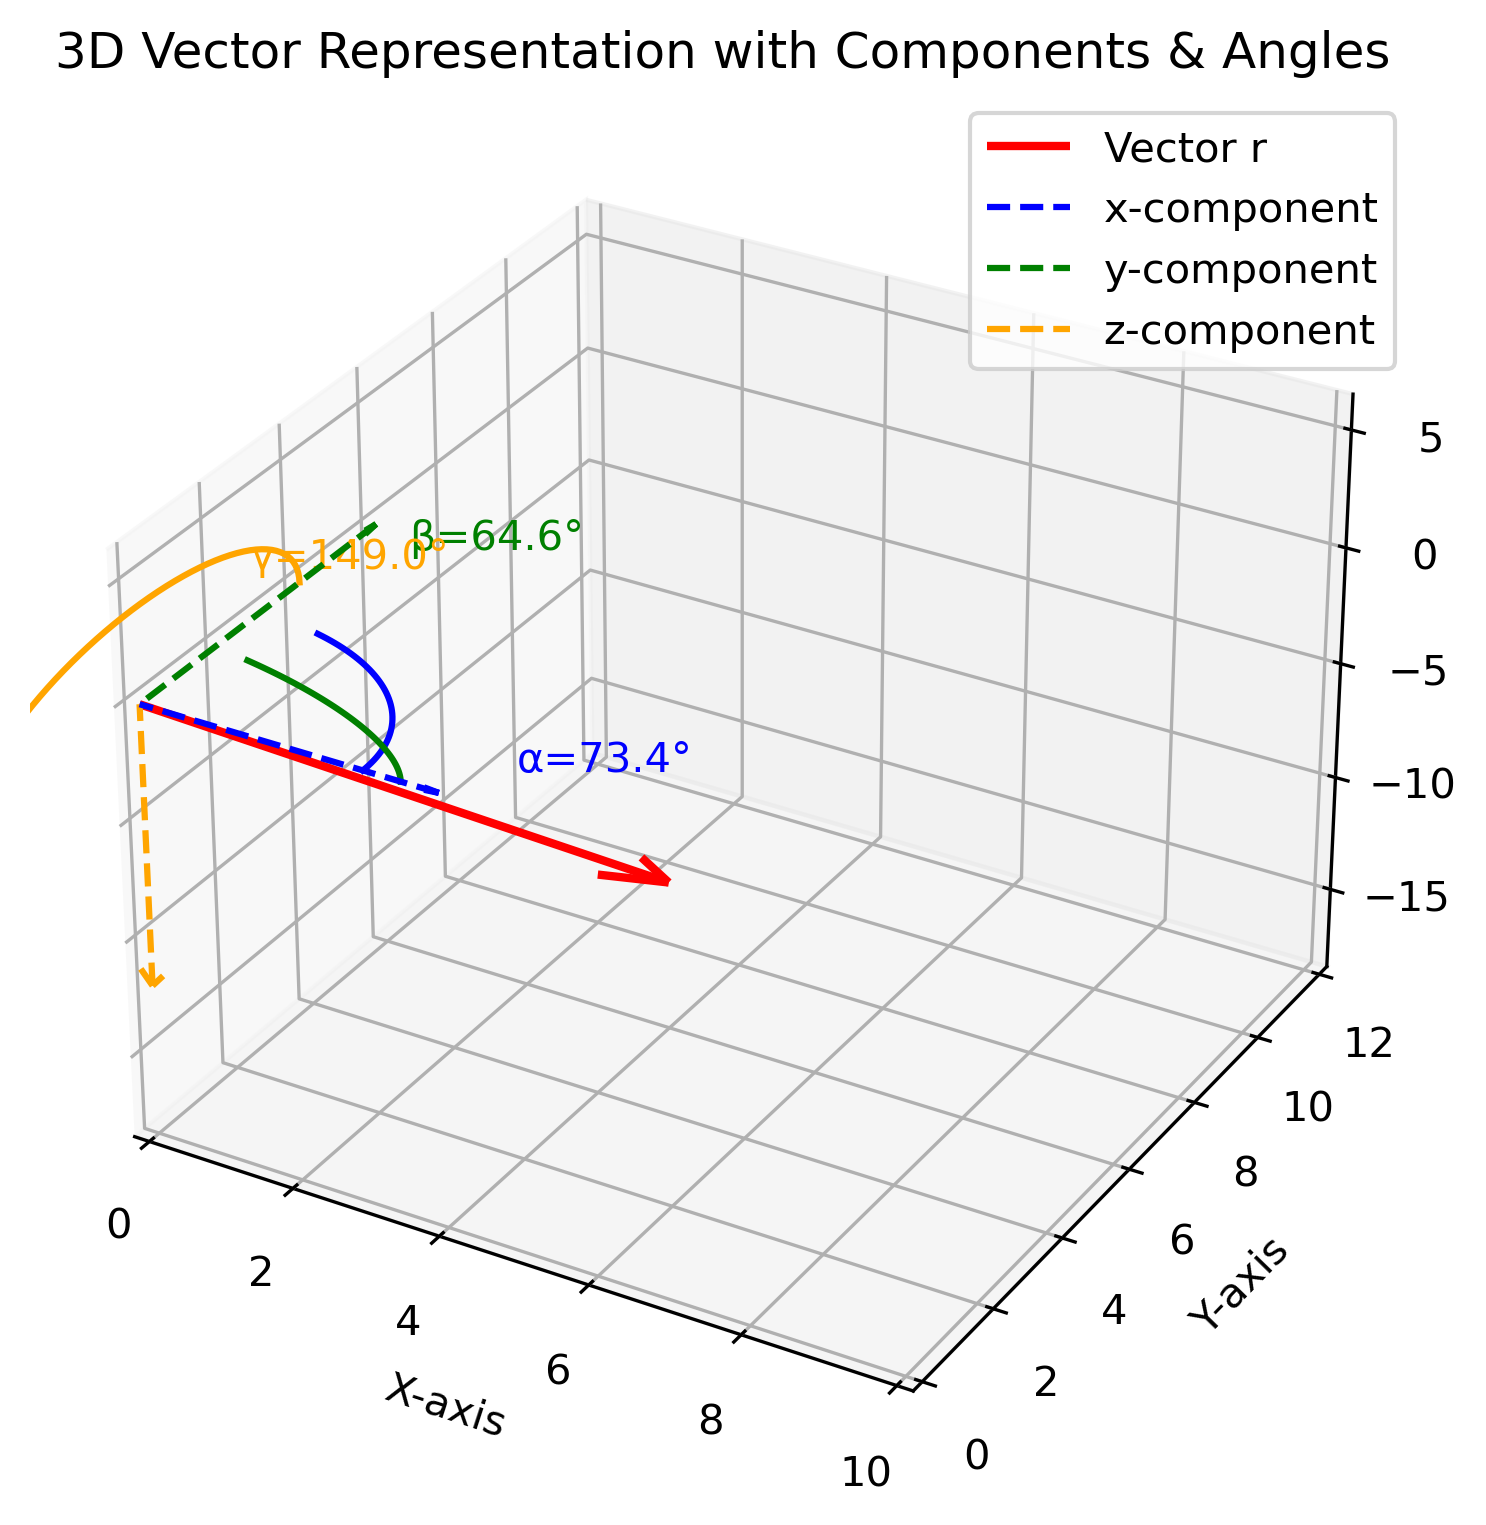
\includegraphics[width=0.5\linewidth]{figs/01.png}
   \caption{}
   \label{}
\end{figure}
\end{frame}

% --------- CODE APPENDIX ---------
\section*{Appendix: Code}

% C program
\begin{frame}[fragile]{C Code: code.c}
\begin{lstlisting}[language=C]
#include <stdio.h>
#include <math.h>

int main() {
    FILE *fp;
    double magnitude, l, m, n;
    double dr1, dr2, dr3;  // direction ratios
    double k;              // normalization factor
    double comp_x, comp_y, comp_z;

    // Open file vector.dat
    fp = fopen("vector.dat", "r");
    if (fp == NULL) {
        printf("Error! Could not open file.\n");
        return 1;
    }

    // Reading magnitude and direction ratios
    fscanf(fp, "%lf %lf %lf %lf", &magnitude, &dr1, &dr2, &dr3);
    fclose(fp);

    // Calculate normalization factor
    k = sqrt(dr1*dr1 + dr2*dr2 + dr3*dr3);

    // Direction cosines
    l = dr1 / k;
    m = dr2 / k;
    n = dr3 / k;

    //  Verify that angle with X-axis is acute
    if (l <= 0) {
        printf("Error: The vector does not make an acute angle with the X-axis.\n");
        return 1;}
\end{lstlisting}
\end{frame}
\begin{frame}[fragile]{C Code: code.c}
\begin{lstlisting}[language=C]
    // Components of vector
    comp_x = magnitude * l;
    comp_y = magnitude * m;
    comp_z = magnitude * n;

    // Display results
    printf("Direction Cosines: l = %.3f, m = %.3f, n = %.3f\n", l, m, n);
    printf("Components of vector r: (%.3f, %.3f, %.3f)\n", comp_x, comp_y, comp_z);
 return 0;
}
\end{lstlisting}
\end{frame}

% Python calling C
\begin{frame}[fragile]{Python: call.py}
\begin{lstlisting}[language=Python]
import subprocess

# Step 1: Create vector.dat automatically
with open("vector.dat", "w") as f:
    f.write("14 2 3 -6\n")   # You can change values here if needed

# Step 2: Compile the C code with -lm (math library)
compile_result = subprocess.run(["gcc", "code.c", "-o", "vector", "-lm"], capture_output=True, text=True)

if compile_result.returncode != 0:
    print("Compilation failed:\n", compile_result.stderr)
else:
    print("Compilation successful. Running program...\n")
    # Step 3: Run the compiled program
    run_result = subprocess.run(["./vector"], capture_output=True, text=True)
    
    # Step 4: Print program output (results or error from C code)
    if run_result.stdout.strip():
        print(run_result.stdout.strip())
    if run_result.stderr.strip():
        print("Runtime error:\n", run_result.stderr.strip())

\end{lstlisting}
\end{frame}

% Python plotting
\begin{frame}[fragile]{Python: plot.py}
\begin{lstlisting}[language=Python]
import numpy as np
import matplotlib.pyplot as plt
from mpl_toolkits.mplot3d import Axes3D

# -----------------------------
# Read magnitude and direction ratios from file
# vector.dat should contain: 14 2 3 -6
# -----------------------------
data = np.loadtxt("vector.dat")
magnitude, a, b, c = data

# Normalize direction ratios → direction cosines
d = np.sqrt(a**2 + b**2 + c**2)
l, m, n = a/d, b/d, c/d

# Vector components (scaled by magnitude)
x, y, z = magnitude * np.array([l, m, n])

# Angles with axes
alpha = np.degrees(np.arccos(l))   # angle with x-axis
beta  = np.degrees(np.arccos(m))   # angle with y-axis
gamma = np.degrees(np.arccos(n))   # angle with z-axis

# -----------------------------
# Verify condition: r makes acute angle with x-axis
# -----------------------------
if alpha >= 90:
    print(f"Vector r does NOT make an acute angle with x-axis (α = {alpha:.2f}°). No figure generated.")
else:
    print(f"Vector r makes an acute angle with x-axis (α = {alpha:.2f}°). Generating figure...")

    # -----------------------------
    # Plot setup (one figure only)
    \end{lstlisting}
\end{frame}

\begin{frame}[fragile]{Python: plot.py}
\begin{lstlisting}[language=Python]
    # -----------------------------
    fig = plt.figure(figsize=(8, 6))
    ax = fig.add_subplot(111, projection='3d')

    # Plot the main vector
    ax.quiver(0, 0, 0, x, y, z, color='r', arrow_length_ratio=0.1, linewidth=2, label="Vector r")

    # Plot projections on axes
    ax.quiver(0, 0, 0, x, 0, 0, color='b', linestyle='dashed', arrow_length_ratio=0.05, label="x-component")
    ax.quiver(0, 0, 0, 0, y, 0, color='g', linestyle='dashed', arrow_length_ratio=0.05, label="y-component")
    ax.quiver(0, 0, 0, 0, 0, z, color='orange', linestyle='dashed', arrow_length_ratio=0.05, label="z-component")

    # Function to draw arc in 3D
    def plot_arc(ax, radius, angle, axis='x', color='k'):
        t = np.linspace(0, np.radians(angle), 50)
        if axis == 'x':
            xs, ys, zs = radius*np.cos(t), radius*np.sin(t), 0*t
        elif axis == 'y':
            xs, ys, zs = radius*np.cos(t), 0*t, radius*np.sin(t)
        else:  # z-axis
            xs, ys, zs = 0*t, radius*np.cos(t), radius*np.sin(t)
        ax.plot(xs, ys, zs, color=color, linewidth=1.5)

    # Draw arcs (different radii to avoid overlap)
    plot_arc(ax, 3, alpha, axis='x', color='b')      # α at radius 3
    plot_arc(ax, 3.5, beta, axis='y', color='g')     # β at radius 3.5
    plot_arc(ax, 4, gamma, axis='z', color='orange') # γ at radius 4

    # -----------------------------
    # Angle labels (separated properly)
\end{lstlisting}
\end{frame}

\begin{frame}[fragile]{Python: plot.py}
\begin{lstlisting}[language=Python]
    # -----------------------------
    ax.text(4.5, 1, 0, f"α={alpha:.1f}°", color='b')      # α label far on +x
    ax.text(1, 5.0, 1, f"β={beta:.1f}°", color='g')       # β label farther on +y
    ax.text(1, 1, 5.2, f"γ={gamma:.1f}°", color='orange') # γ label higher on +z

    # -----------------------------
    # Axes labels & limits
    # -----------------------------
    ax.set_xlim([0, max(0, x) + 6])
    ax.set_ylim([0, max(0, y) + 6])
    ax.set_zlim([min(0, z) - 6, max(0, z) + 6])

    ax.set_xlabel("X-axis")
    ax.set_ylabel("Y-axis")
    ax.set_zlabel("Z-axis")
    ax.set_title("3D Vector Representation with Components & Angles")

    ax.legend()

    # Save the figure and show it
    plt.savefig("vector_plot.png", dpi=300, bbox_inches='tight')
    plt.show()
\end{lstlisting}
\end{frame}
\end{document}
